\documentclass[11pt,a4paper]{article}
\usepackage {amsmath, amssymb, amsfonts}
\usepackage {graphics}
\usepackage {graphicx}
\usepackage{placeins}

\usepackage{hyperref}
\usepackage{float}
\usepackage{csquotes}
\usepackage[linesnumbered, ruled,longend]{algorithm2e}
\usepackage{amsmath}
\usepackage{bbm}
\usepackage[scaled]{helvet}
\usepackage[cm]{sfmath}
\usepackage[T1]{fontenc}
\renewcommand{\familydefault}{\sfdefault}
\usepackage[doublespacing]{setspace}
\usepackage{sansmath}
 %\usepackage{algorithmicx,algpseudocode}
\usepackage{anysize}
\usepackage{siunitx}
\usepackage{mathtools}
\usepackage{multicol}
\usepackage{todonotes}

%\usepackage{lineno}
%\linenumbers

\topmargin 0.0cm
\oddsidemargin 0.2cm
\textwidth 16cm 
\textheight 23cm
\footskip 1.0cm

\renewcommand\Re{\operatorname{Re}}
\renewcommand\Im{\operatorname{Im}}
\DeclareMathOperator{\argmax}{argmax}
\DeclareMathOperator{\argmin}{argmin}

\newtheorem{lemma}{Lemma}
\newtheorem{theorem}{Theorem}
\newtheorem{proposition}{Proposition}
\newtheorem{remark}{Remark}
\newtheorem{corollary}{Corollary}

\usepackage{color,soul}
\newcommand{\nonl}{\renewcommand{\nl}{\let\nl\oldnl}}% Remove line number for one line
\newcommand{\mymathsf}[1]{\mbox{\sansmath$\mathsf{#1}$}}
\SetKw{KwGoTo}{go to}

\usepackage[backend=bibtex, style=numeric, sorting=none]{biblatex} 
\addbibresource{BK_chaos} 

\begin{document}
\title{Chaos in small microbial communities}
\author{Behzad D. Karkaria$^{1}$ Kiran R. Patil$^{1}$\\
\normalsize{$^{1}$MRC Tox}\\
\\
\normalsize{$^\ast$To whom correspondence should be addressed;}\\
\normalsize{E-mail: }
}
\date{}

\maketitle
\begin{abstract}
    Genome scale metabolic model reconstructions are relatively poor at predicting species viability in specified media. Methods such as gap-filling, require experimental data to identify which metabolic reactions should be added to achieve species growth. However, this therefore requires \textit{in vitro} screening of each species in different media environments. We have developed a machine learning pipeline that can predict the viability of a microbial species in a given defined media. We propose that this pipeline can be used to perform automatic gap-filling, to improve the output of existing automated metabolic reconstruction frameworks.
\end{abstract}

\section{Introduction}
\dots
\section{Results}
GSMM reconstruction pipelines such as metaGEM, take the genome sequece of a species and use databases of annotated genes to construct a network of reactions that describe the organisms metabolism. Incomplete genome sequences and incomplete annotation databases result in missing reactions (gaps). Gapfilling methods take a defined media that the species is known to grow in, and adds reactions to the model that would enable such growth. 
\par
When performing a large number of genome reconstructions, gapfilling is generally performed using a "complete media". T
\par
Figure x shows a dendrogram of species, coupled with a heatmap showing their growth rates in different defined media. The dendrogram is created by hierarchical clustering, using reactions in the GSMMs as features. The heatmap shows patterns of growth between related organisms. This figure provides a good indication that GSMMs include features that can be used in machine learning techniques to predict growth.

\begin{figure}[p]
    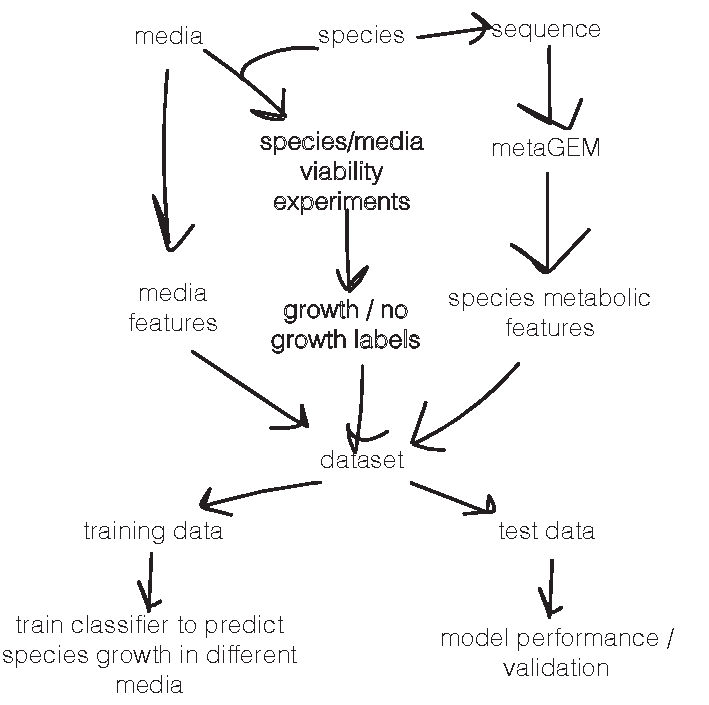
\includegraphics[width=\textwidth]{figures/FIG_pipeline.pdf}
    \caption{}
    \label{fig:FIG_pipeline}
 \end{figure}

\begin{figure}[p]
    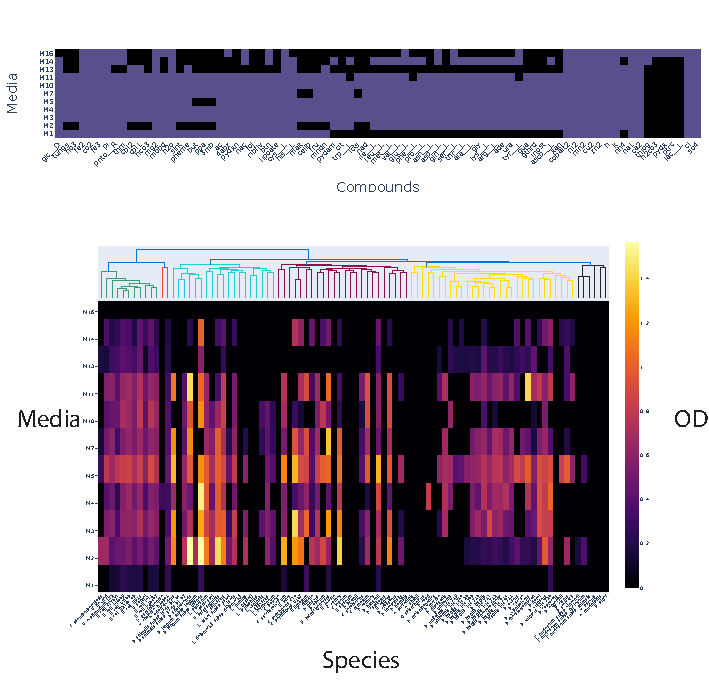
\includegraphics[width=\textwidth]{figures/FIG_dataset.pdf}
    \caption{}
    \label{fig:FIG_dataset}
 \end{figure}
 
 \begin{figure}[p]
    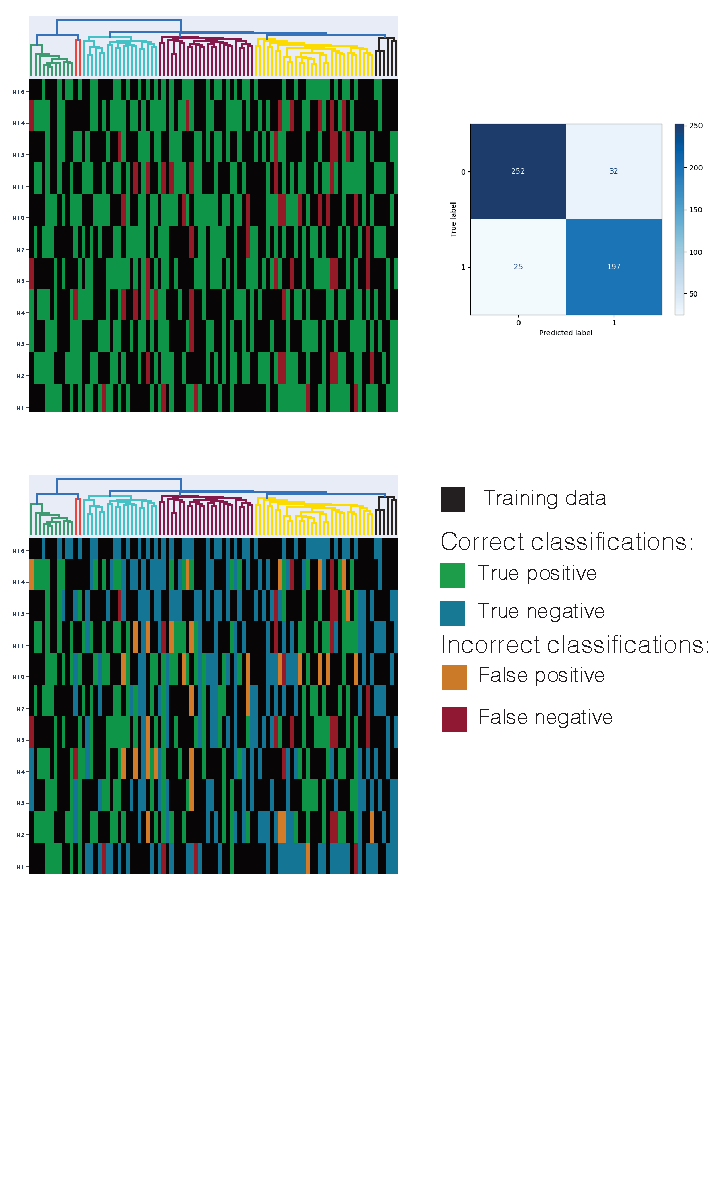
\includegraphics[width=\textwidth]{figures/FIG_classifier_dendrogram.pdf}
    \caption{}
    \label{fig:FIG_classifier_dendrogram}
 \end{figure}


\section{Methods}

\end{document}